\documentclass{article}



\usepackage{arxiv}

\usepackage[utf8]{inputenc} % allow utf-8 input
\usepackage[T1]{fontenc}    % use 8-bit T1 fonts
\usepackage{hyperref}       % hyperlinks
\usepackage{url}            % simple URL typesetting
\usepackage{booktabs}       % professional-quality tables
\usepackage{amsfonts}       % blackboard math symbols
\usepackage{nicefrac}       % compact symbols for 1/2, etc.
\usepackage{microtype}      % microtypography
\usepackage{lipsum}		% Can be removed after putting your text content
\usepackage{graphicx}
\usepackage{natbib}
\usepackage{doi}
\usepackage{graphicx}
\usepackage{parskip}
\usepackage{float}




\title{Predicting the Influence of Internet Culture on Kalshi Spending: An LLM Agent Approach to What will Shaquille O'Neal say during Inside the NBA?}

%\date{September 9, 1985}	% Here you can change the date presented in the paper title
%\date{} 					% Or removing it

\author{
    Bowie Vaughan \\
    \texttt{bowievaughan@gmail.com} \\
    \And
    Aaron Grinberg \\
    \texttt{aarongrinberg@gmail.com} \\
}

% Uncomment to remove the date
%\date{}

% Uncomment to override  the `A preprint' in the header
\renewcommand{\headeright}{}
\renewcommand{\undertitle}{}
\renewcommand{\shorttitle}{\textit{} PREDICTING THE INFLUENCE OF INTERNET CULTURE ON
KALSHI SPENDING}

\date{\textit{Institute for Computing in Research} \\[4mm] \today}

%%% Add PDF metadata to help others organize their library
%%% Once the PDF is generated, you can check the metadata with
%%% $ pdfinfo template.pdf
\hypersetup{
pdftitle={A template for the arxiv style},
pdfsubject={q-bio.NC, q-bio.QM},
pdfauthor={David S.~Hippocampus, Elias D.~Striatum},
pdfkeywords={First keyword, Second keyword, More},
}

\begin{document}
\maketitle

\begin{abstract}
	Prediction markets increasingly list betting lines influenced by the internet and meme culture alongside traditional politics, financial, and sports markets. This research examines whether a market's genre of betting, influences the trading volume it attracts on Kalshi. Using an LLM built from the open source tool Langflow, and powered by the open source AI, "LLama," 1,433 betting lines were categorized as "Meme," "Serious," and "Grey." These categories were determined by human feedback, theory, and real world events all through the LLM. These categories were also further labeled "sports" and "non-sports." Ordinary least squares regression was used to model trading volume as a function of category, bet type, and market duration (days). Relative to meme labeled markets, serious markets were associated with significantly higher volume (p < .001 for Models 2 and 3). Sports bets were related to less volume compared to non sports bets across the models, and longer market duration was associated with higher volume. These preliminary results indicate that markets tied to consequential real world events attract more capital than meme driven markets. 
\end{abstract}
%%% Maybe add an asterik next to Langflow to tell the audience the name of the LLM -meorser-

% keywords can be removed
\keywords{First keyword \and Second keyword \and More}


\section{Introduction}
Prediction markets grow year after year as the varying markets to bet on expand. One of the main selling points, is the ability to bet on absurdity, memes, and implausibility. Prediction markets include bets on predicting what Trump will say on his next speech, if GTA VI will ever release, and if we can expect a thunderstorm tomorrow. Little is known whether internet culture markets command real trading volume comparable to more conventional, traditional markets, or whether their popularity is mostly noise with minimal capital behind it. 

This paper sets out to answer that question using an original data set of 1,433 Kalshi betting lines, classified by an LLM and sorted into three categories "Meme," "Serious," and "Grey." Each category was further evaluated for whether it constituted a sports bet, since sports make up the largest single category of listings, and also the control variable of duration for how long the betting line stayed open on the market. Using this classification, the paper tests whether a market's cultural framing predicts the amount of volume it attracts, and whether that relationship changes once sports and non-sports markets are considered separately and market duration.

\section{Methods}
A brief overview of the methods used throughout the research conducted include the process of building an LLM to process betting lines, and output into the three categories of "Meme," "Serious," and "Grey." The data set used for this research is from huggingface by the author Deniz Zorlu\footnote {Zorlu, D.
kalshi-filtered. Hugging Face. Retrieved from \url{dzorlu/kalshi-filtered}.} and includes 1,433 rows of betting lines, dates, tickers, and more.
%%% need to add a footnote here for Deniz
\label{sec:headings}

%%%\lipsum[4] See Section \ref{sec:headings}.

\subsection{Category Definitions}
To keep the LLM's classification consistent, each category had specific defined criteria the agent followed per each betting line.

\textbf{Meme}
markets were defined as bets tied to pop and internet culture, celebrity behaviors, unfathomable events, or events with no real world or political consequence (e.g., celebrity breakups, Twitter/X drama, joke crypto tokens, religious internet memes, crazy ideas). Betting on these primarily represents signaling involvement with pop-cultural discourse; earnest or ironically.

\textbf{Serious}
markets were defined as bets tied to real world financial and political events, Standard political, macroeconomic, geopolitical, or highly consequential real-world events (e.g., presidential elections, central bank rates, major legislation, sport questions with clear real stakes like a golden boot winner). Betting on these primarily represents an individual using knowledge to make money.

\textbf{Grey}
markets that are generally niche, unusual, uncommon, or technically complex markets that don't cleanly fit Serious or Meme (e.g., obscure scientific replication studies, minor localized weather data, hypothetical sports scenarios). Betting on these could equally reflect hyper specific knowledge or an irregular bet.  

%%%source llama used to create prompts
\subsection{Creating the LLM agent}
To start the data collection process, an LLM agent was necessary in sorting the data in an efficient manner. Using the app Langflow\footnote{Langflow. (2026
). Langflow: An open-source visual framework for building LLM applications. \url{https://www.langflow.org}.}, which is a free agent building service, and an API key\footnote{API access provided via GroqCloud. \url{https://groq.com}.} for the ai model llama-3.1-8b-instant\footnote{Meta AI. (2024). Llama 3.1 (8B Instant). \url{https://ai.meta.com/llama/}.},for the ai model llama-3.1-8b-instant, the first variation of meorser (the category sorting agent, shortened for "MemeorSerious") was built. The first variation was unique in the way that it broke down each betting line you fed it and provided an in depth reason as to why said betting fell into each category. In order to ensure more accurate results, I fed it 50+ markets and had it label them to what category fit best. I included examples of what to do, and what not to do in my prompt. Through vibe based prompting and constant adjustments, eventually a consistent working agent was formed. After accurately representing what each category the various markets fell into, the next variation was created. The second variation of meorser, reads large .csv files and outputs them into a neatly organized data table that additionally includes the category for each betting line, and also the classification of sports and non-sports.  
 %%%footnote for groqcloud for api key
\subsection{Data Collection}
For data collection, the dataset was processed through meorser and the output contained the added columns of category and sports/non-sports. The results are shown in the two histograms below. The first histogram represents the \% of each category in the dataset and the second histogram represents the average volume per each category. 


\begin{figure}[H]
    \centering
    \begin{minipage}{0.6\textwidth}
        \centering
        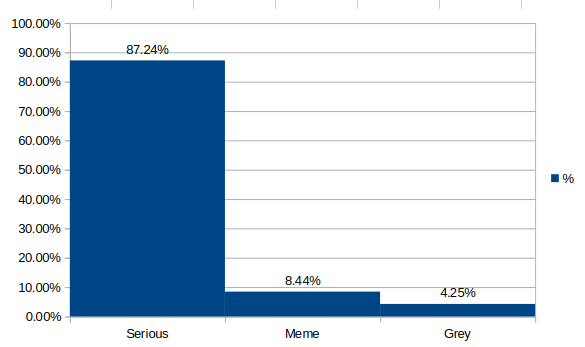
\includegraphics[width=\linewidth]{histogrammeorser.png}
        \caption{Percentage of markets by category (Meme, Serious, Grey).}
        \label{fig:histogrammeorser}
    \end{minipage}
    \hfill
    \begin{minipage}{0.6\textwidth}
        \centering
        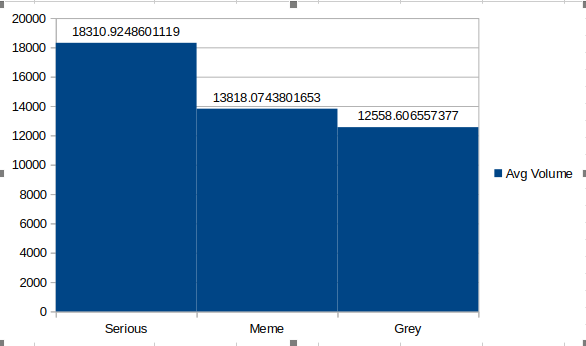
\includegraphics[width=\linewidth]{Volumepermeorser.png}
        \caption{Average trading volume by category.}
        \label{fig:Volumepermeorser}
    \end{minipage}
\end{figure}

%%% set to roughly .48\textwidth if we wanted side by side histograms

%\subsubsection{Headings: third level}
%\lipsum[6]

%\paragraph{Paragraph}
%\lipsum[7]



\section{Preliminary Results with OLS Regression}
To examine whether a market's category influences the trading volume it receives on Kalshi, three sequential OLS regression models were built using the 1,433 betting lines. Data processing was conducted using pandas\footnote{McKinney, W. (2010). Data structures for statistical computing in Python. \url{https://pandas.pydata.org}.}, and regression models were estimated using the statsmodels.formula.api module\footnote{Seabold, S., \& Perktold, J. (2010). Statsmodels. \url{https://www.statsmodels.org}.}. Trading volume was used as the dependent variable across all models, with "meme" serving as the reference category. Model 1 included only the category classifications (Grey and Serious, relative to Meme). Model 2 introduced the sports betting classification. Model 3 introduced market duration (in days), to control for markets accumulating volume over longer amounts of times, regardless of category.
\label{sec:others}

\subsection{Models}
Model 1 tested the amount of volume in Grey and Serious markets and whether that differed from Meme markets. The results were statistical insignificant (Grey: B = -1,259, SE = 12,600; Serious: B = 4,492, SE = 7,649). Meaning this model was not sufficient in finding meaningful volume distinctions.  
Model 2 introduced the sports betting control, and revealed two statistically significant relationships. Serious markets were associated with substantially higher trading volume then Meme markets (B = 46,270, p<.001), suggesting that Serious markets attract significantly more capital then Meme-driven markets. Conversely, sports bet were associated with greatly reduced predicted volume compared to non-sports markets (B = -52,210, SE = 5,458). Grey markets remain statistically insignificant. 
Model 3 introduced market duration (in days), which displays three statistically significant results. Market duration has a positive correlation to predicted volume, regardless of category, by an estimated increase of 607 units of volume per day. When controlling for market duration, the predicted volume of sports bets significantly increases (B = -34,890, SE = 5,750). The volume advantages of Serious markets compared to Meme markets is not defined by market duration (B = 44,160, SE = 8,423) unlike sports bets.
\begin{figure}[H]
    \centering
    \includegraphics[width=0.8 \linewidth]{actualdatatable1.png}
    \caption{Regression results for Model 1, Model 2, and Model 3. Coefficients represent measures of volume.}
    \label{fig:placeholder}
\end{figure}


\section{Conclusion}

\subsection{Limitations}
The limitations throughout this research included the dataset, being from a third party source not directly from the Kalshi API. Also, more data and datasets would have been ideal to identify more patterns and receive more accurate results. However, the most relevant limitation is subjectivity. The LLM created for the purpose of this paper is not a perfect machine, some if not many of the categories it labeled as Serious, Meme, and Grey are subjective and could be identified as a different category by another source. The Grey category was implemented in an attempt to subside the subjectivity.   
\subsection{Discussion}
The media tends to lean one way when it comes to trends, specifically internet trends. Because of Kalshi being accessible to people as early as 18 year of age, and the constant attempt of older generation figures and politicians trying to win over the younger audience (Making jokes, buying into pop culture), the amount of volume in Meme categories did not comprehensively reflect that in this research. However, this research did show that sports bets tend to be less popular on Prediction Markets, implying that the predicted volume is spread out into other categories. 

\section{Acknowledgments}

I would like to thank my mentor, Aaron Grinberg, who guided and supported me throughout this
project. I would also like to thank the Institute for Computing in Research for providing this opportunity. 


\begin{thebibliography}{9}

	\bibitem{zorlu2024}
	Zorlu, D. (2026).
	\newblock \emph{Kalshi Prediction Market Dataset}.
	\newblock Hugging Face.
	\newblock \url{https://huggingface.co/datasets/dzorlu/kalshi-filtered}

	\bibitem{langflow}
	Langflow. (2026).
	\newblock \emph{Langflow: An open-source visual framework for building LLM applications}.
	\newblock \url{https://www.langflow.org}

	\bibitem{groq2024}
	GroqCloud. (2026).
	\newblock \emph{GroqCloud: Low-latency inference platform}.
	\newblock \url{https://groq.com}

	\bibitem{meta2024}
	Meta AI. (2026).
	\newblock \emph{Llama 3.1 (8B Instant)}.
	\newblock \url{https://ai.meta.com/llama/}

    \bibitem{mckinney2010pandas}
	McKinney, W. (2010).
	\newblock Data structures for statistical computing in Python.
	\newblock \emph{Proceedings of the 9th Python in Science Conference}.
	\newblock \url{https://pandas.pydata.org}

	\bibitem{seabold2010statsmodels}
	Seabold, S., \& Perktold, J. (2010).
	\newblock Statsmodels.
	\newblock \emph{Proceedings of the 9th Python in Science Conference}.
	\newblock \url{https://www.statsmodels.org}

\end{thebibliography}
%\footnote{Sample of the first footnote.}




\end{document}
